% ============================================================================
% Chapitre 4 — Conception et architecture
% ============================================================================
\chapter{Conception et architecture}

\section*{Introduction}

Ce chapitre est le cœur technique du rapport. Il décrit l'architecture
microservices de \caimp{}, le modèle de données, les flux de traitement principaux
et les décisions de conception qui ont guidé le développement. Chaque choix
architectural est justifié par rapport aux alternatives évaluées.

\section{Choix architectural : microservices vs. monolithe}

Face aux besoins de \caimp{}, deux approches architecturales ont été évaluées :
un monolithe modulaire et une architecture microservices. Le tableau~\ref{tab:arch-choice}
synthétise l'analyse comparative.

\begin{table}[H]
\centering
\caption{Comparaison monolithe vs. microservices pour \caimp{}}
\label{tab:arch-choice}
\small
\begin{tabularx}{\textwidth}{lXX}
\toprule
\textbf{Critère} & \textbf{Monolithe modulaire} & \textbf{Microservices} \\
\midrule
Déploiement       & Simple (un processus)         & Complexe (Docker Compose) \\
Scalabilité       & Verticale uniquement          & Horizontale par service \\
Isolation pannes  & Un crash affecte tout         & Dégradation gracieuse \\
Langages mixtes   & Impossible                    & Possible (Go + Python) \\
Découplage IA     & LLM dans le processus API     & Worker dédié, indépendant \\
Évolutivité       & Refactoring difficile         & Ajout de services isolé \\
\bottomrule
\end{tabularx}
\end{table}

L'architecture microservices a été retenue pour trois raisons déterminantes :
(1)~le moteur de prévision Holt-Winters et l'inférence LLM sont des tâches
de calcul intensif qui ne doivent pas bloquer les \api{} de requête ;
(2)~le télétransmetteur Go bénéficie des goroutines pour l'ingestion
concurrente sans les limitations du GIL Python ;
(3)~l'ajout futur de nouvelles sources de métriques (Kubernetes, AWS CloudWatch)
ne nécessitera pas de modifier les services existants.

\section{Architecture globale}

La plateforme \caimp{} est composée de 19 services conteneurisés organisés en
quatre couches fonctionnelles :

\begin{description}[leftmargin=2cm]
  \item[Couche d'ingestion] Reçoit les métriques des agents (\servicename{telemetry-writer},
    \servicename{splunk-hec-bridge}) et les changements (\servicename{change-tracker}).
  \item[Couche d'événements] Bus NATS JetStream assurant la communication
    asynchrone entre tous les services.
  \item[Couche de traitement] Services consommateurs (\servicename{ai-worker},
    \servicename{alert-engine}, \servicename{forecast-engine},
    \servicename{correlation-engine}) traitant les événements de manière découplée.
  \item[Couche de présentation] APIs REST (\servicename{query-api},
    \servicename{admin-api}), WebSocket Gateway et frontend React.
\end{description}

\begin{landscape}
\begin{figure}[H]
\centering
\resizebox{\linewidth}{!}{%
\begin{tikzpicture}[
  % ── Styles ──────────────────────────────────────────────────────
  svc/.style   = {draw=NavyBlue,    fill=NavyBlue!10,     rounded corners=4pt,
                  minimum width=3.2cm, minimum height=0.9cm,
                  font=\normalsize\bfseries, align=center},
  agent/.style = {draw=SuccessGreen, fill=SuccessGreen!12, rounded corners=4pt,
                  minimum width=3.2cm, minimum height=0.9cm,
                  font=\normalsize\bfseries, align=center},
  store/.style = {draw=TealBlue,    fill=TealBlue!10,     rounded corners=4pt,
                  minimum width=3.4cm, minimum height=0.9cm,
                  font=\normalsize\bfseries, align=center},
  bus/.style   = {draw=AccentOrange, fill=AccentOrange!12, rounded corners=6pt,
                  minimum width=15.0cm, minimum height=1.0cm,
                  font=\large\bfseries, align=center,
                  text=AccentOrange!80!black},
  proxy/.style = {draw=DarkGray!70, fill=DarkGray!10,     rounded corners=4pt,
                  minimum width=15.0cm, minimum height=0.9cm,
                  font=\large\bfseries, align=center},
  layer/.style = {font=\small\bfseries\color{NavyBlue!70},
                  anchor=west, inner sep=0},
  arr/.style   = {-{Stealth[length=6pt]}, thick, draw=NavyBlue!60},
  darr/.style  = {-{Stealth[length=6pt]}, thick, draw=NavyBlue!35, dashed},
]

% ── Bandes de couches (background) ──────────────────────────────
\begin{scope}[on background layer]
  \fill[SuccessGreen!6,  rounded corners=5pt] (-2.4, 8.9) rectangle (13.8, 10.1);
  \fill[NavyBlue!5,      rounded corners=5pt] (-2.4, 7.4) rectangle (13.8,  8.8);
  \fill[AccentOrange!6,  rounded corners=5pt] (-2.4, 5.9) rectangle (13.8,  7.3);
  \fill[NavyBlue!5,      rounded corners=5pt] (-2.4, 4.4) rectangle (13.8,  5.8);
  \fill[TealBlue!5,      rounded corners=5pt] (-2.4, 2.9) rectangle (13.8,  4.3);
  \fill[NavyBlue!5,      rounded corners=5pt] (-2.4, 1.4) rectangle (13.8,  2.8);
  \fill[DarkGray!6,      rounded corners=5pt] (-2.4, 0.1) rectangle (13.8,  1.3);
\end{scope}

% ── Étiquettes de couche ────────────────────────────────────────
\node[layer] at (-2.3, 9.5)  {Serveurs};
\node[layer] at (-2.3, 8.1)  {Ingestion};
\node[layer] at (-2.3, 6.6)  {Bus};
\node[layer] at (-2.3, 5.1)  {Traitement};
\node[layer] at (-2.3, 3.6)  {Données};
\node[layer] at (-2.3, 2.1)  {Présentation};
\node[layer] at (-2.3, 0.7)  {Accès};

% ── Ligne 1 : Serveurs surveillés ───────────────────────────────
\node[agent] (a1) at (1.6,  9.5) {Serveur A};
\node[agent] (a2) at (5.6,  9.5) {Serveur B};
\node[agent] (a3) at (9.6,  9.5) {Serveur C};

% ── Ligne 2 : Ingestion ─────────────────────────────────────────
\node[svc] (tw)  at (1.6,  8.1) {Telemetry Writer};
\node[svc] (hec) at (5.6,  8.1) {HEC Bridge};
\node[svc] (ct)  at (9.6,  8.1) {Change Tracker};

% ── Ligne 3 : Bus NATS ──────────────────────────────────────────
\node[bus] (nats) at (5.7, 6.6) {NATS JetStream};

% ── Ligne 4 : Workers ───────────────────────────────────────────
\node[svc] (aiw) at (0.8,  5.1) {AI Worker};
\node[svc] (ale) at (3.8,  5.1) {Alert Engine};
\node[svc] (fce) at (7.0,  5.1) {Forecast Engine};
\node[svc] (cor) at (10.5, 5.1) {Correlation Engine};

% ── Ligne 5 : Données ───────────────────────────────────────────
\node[store] (pg)    at (2.4,  3.6) {PostgreSQL};
\node[store] (redis) at (6.2,  3.6) {Redis :6379};
\node[store] (oll)   at (10.5, 3.6) {Ollama :11434};

% ── Ligne 6 : APIs / Frontend ───────────────────────────────────
\node[svc] (fe)   at (0.8,  2.1) {Frontend :3000};
\node[svc] (qapi) at (3.8,  2.1) {Query API :8002};
\node[svc] (adm)  at (7.0,  2.1) {Admin API :8001};
\node[svc] (wsg)  at (10.5, 2.1) {WS Gateway};

% ── Ligne 7 : Nginx ─────────────────────────────────────────────
\node[proxy] (nginx) at (5.7, 0.7) {Nginx — Reverse Proxy :80 / :443};

% ── Flèches ─────────────────────────────────────────────────────

% Serveurs → Ingestion
\draw[arr] (a1) -- (tw);
\draw[arr] (a2) -- (hec);
\draw[arr] (a3) -- (ct);

% Ingestion → NATS
\draw[arr] (tw)  -- (nats);
\draw[arr] (hec) -- (nats);
\draw[arr] (ct)  -- (nats);

% NATS → Workers
\draw[arr] (nats.south) -- (aiw.north);
\draw[arr] (nats.south) -- (ale.north);
\draw[arr] (nats.south) -- (fce.north);
\draw[arr] (nats.south) -- (cor.north);

% Workers → Données
\draw[arr] (aiw.south) -- (pg.north);
\draw[arr] (ale.south) -- (redis.north);
\draw[arr] (fce.south) -- (pg.north);
\draw[arr] (cor.south) -- (oll.north);
\draw[darr] (aiw.south) to[out=-70, in=110] (oll.north);

% Données → APIs
\draw[arr]  (pg.south) -- (qapi.north);
\draw[arr]  (pg.south) to[out=-110, in=90] (fe.north);
\draw[arr]  (pg.south) to[out=-80,  in=90] (adm.north);
\draw[darr] (nats.south) to[out=-5, in=90] (wsg.north);

% APIs → Nginx
\draw[arr] (fe.south)   -- (nginx.north);
\draw[arr] (qapi.south) -- (nginx.north);
\draw[arr] (adm.south)  -- (nginx.north);
\draw[arr] (wsg.south)  -- (nginx.north);

\end{tikzpicture}
}%
\caption{Architecture globale de la plateforme \caimp{} — 7 couches, 19 services}
\label{fig:arch-global}
\end{figure}
\end{landscape}

\section{Fonctionnement de l'architecture — flux de bout en bout}

La figure~\ref{fig:arch-global} présente la structure statique de la plateforme.
Cette section décrit son fonctionnement dynamique : comment les données traversent
chaque couche, depuis la collecte sur le serveur surveillé jusqu'à l'affichage
d'une explication en langage naturel dans le navigateur de l'opérateur.

% ─────────────────────────────────────────────────────────────────────────────
\subsection{Flux 1 — Collecte et ingestion des métriques}

L'agent \caimp{} est un processus Python déployé sur chaque serveur cible.
Toutes les 15 secondes, il lit les indicateurs système (\textsc{cpu}, mémoire,
disque) via la bibliothèque \texttt{psutil} et les encode au format
\textsc{otlp}/HTTP (protobuf). Les données sont transmises au
\servicename{Telemetry Writer} (port 4318), service Go qui :

\begin{enumerate}
  \item \textbf{Reçoit} le batch OTLP et extrait les points de métrique ;
  \item \textbf{Persiste} les valeurs dans la table \texttt{metrics}
        (hypertable TimescaleDB) via une insertion groupée (\texttt{COPY}) ;
  \item \textbf{Détecte} les anomalies en parallèle grâce à trois algorithmes
        (seuil statique, Z-score, taux de variation) ;
  \item \textbf{Publie} chaque anomalie détectée sur le sujet NATS
        \texttt{anomaly.detected.\{org\_id\}.\{severity\}}.
\end{enumerate}

En parallèle, l'agent exécute quatre \textit{reporters} de changements
qui surveillent en continu les événements Docker, les installations de paquets,
les connexions SSH et les tâches cron. Ces événements sont envoyés au
\servicename{Change Tracker} (port 8011), qui les inscrit dans la table
\texttt{change\_events} et les publie sur le sujet \texttt{change.detected.>}.

% ─────────────────────────────────────────────────────────────────────────────
\subsection{Flux 2 — Analyse IA et explication de l'anomalie}

Dès qu'un message \texttt{anomaly.detected.*} arrive sur le bus NATS,
\textbf{deux services consommateurs} s'activent de manière indépendante :

\paragraph{AI Worker} Ce service abonne la file \texttt{ANOMALIES} et, pour
chaque anomalie :

\begin{enumerate}
  \item Interroge PostgreSQL pour récupérer les 30 dernières minutes de métriques
        (contexte historique du serveur) ;
  \item Interroge pgvector par similarité cosinus pour retrouver les runbooks et
        les incidents passés les plus similaires (\textit{Retrieval-Augmented
        Generation, \rag{}}) ;
  \item Construit un prompt structuré ciblant un développeur non DevOps, en
        langage naturel, et l'envoie à Ollama (\textsc{llm} Llama~3.1~8B) ;
  \item Valide le JSON retourné par le modèle, l'insère dans
        \texttt{ai\_explanations}, puis publie un message
        \texttt{ai.explanation.ready.*} sur NATS.
\end{enumerate}

\paragraph{Correlation Engine} Ce service effectue une analyse causale en
parallèle :

\begin{enumerate}
  \item Interroge \texttt{change\_events} dans la fenêtre $[t-30\text{min},\,t]$
        pour le même serveur ;
  \item Score chaque changement candidat par la formule
        $s = e^{-0.1 \cdot \Delta t} \times w_{\text{type}}$
        (décroissance temporelle × poids du type de changement) ;
  \item Envoie les 3 premiers candidats à Ollama avec le contexte de l'anomalie
        pour obtenir un narratif causal en langage naturel ;
  \item Persiste le résultat dans \texttt{root\_cause\_analyses} et publie un
        message \texttt{rootcause.ready.*} sur NATS.
\end{enumerate}

% ─────────────────────────────────────────────────────────────────────────────
\subsection{Flux 3 — Prévision des ressources}

Le \servicename{Forecast Engine} fonctionne de manière entièrement autonome,
indépendamment des anomalies. Il exécute deux boucles périodiques :

\begin{description}[leftmargin=2cm]
  \item[Boucle de prévision (toutes les 30~min)] Pour chaque combinaison
    serveur/métrique, récupère les 6 dernières heures de données, applique
    le lissage exponentiel double de Holt-Winters, génère 24 points de
    prévision horaire avec intervalles de confiance à $\pm 1.28\sigma$,
    calcule le \textit{time-to-critical} (heure prévue de franchissement du
    seuil de 90~\%), demande un narratif à Ollama, et persiste le tout dans
    \texttt{server\_forecasts}.
  \item[Boucle d'évaluation (toutes les 60~min)] Compare les prévisions
    passées aux valeurs réelles, calcule l'erreur absolue moyenne (\textsc{mae}),
    et enrichit le prochain prompt LLM de la précision historique du modèle
    pour calibrer le niveau de confiance exprimé.
\end{description}

% ─────────────────────────────────────────────────────────────────────────────
\subsection{Flux 4 — Mise à jour en temps réel du navigateur}

Le \servicename{WS Gateway} maintient des connexions WebSocket persistantes
avec tous les navigateurs connectés. Il souscrit aux sujets NATS suivants :

\begin{itemize}
  \item \texttt{anomaly.detected.>} — affiche l'alerte dans le fil d'événements ;
  \item \texttt{ai.explanation.ready.>} — met à jour la carte d'explication IA ;
  \item \texttt{rootcause.ready.>} — met à jour l'analyse causale ;
  \item \texttt{forecast.critical.>} — déclenche une notification urgente.
\end{itemize}

Dès qu'un message arrive sur l'un de ces sujets, le gateway le distribue en
\textit{fan-out} à tous les clients WebSocket de l'organisation concernée
(isolation multi-tenant respectée). Le tableau de bord se rafraîchit ainsi
sans aucun \textit{polling} — la latence entre détection et affichage est
inférieure à 3 secondes.

% ─────────────────────────────────────────────────────────────────────────────
\subsection{Flux 5 — Requête utilisateur depuis le tableau de bord}

Lorsqu'un opérateur ouvre le tableau de bord, le navigateur envoie une requête
\texttt{GET /api/v1/dashboard/summary} au \servicename{Query API} (via Nginx).
Celui-ci :

\begin{enumerate}
  \item Récupère les statuts serveurs et les dernières métriques (cache Redis 30~s) ;
  \item Agrège les anomalies des dernières 24~heures ;
  \item Consulte les prévisions à risque (\textit{time\_to\_critical} $\leq$ 24~h) ;
  \item Récupère les dernières analyses de cause racine depuis
        \texttt{root\_cause\_analyses} ;
  \item Construit et retourne la réponse structurée :
        \textit{overall\_status}, \textit{potential\_issues} et
        \textit{recommended\_actions}.
\end{enumerate}

L'interface présente directement le résultat sous forme de
\og{}tableau de bord orienté réponses\fg{} : statut global, problèmes
potentiels triés par criticité, et actions recommandées numérotées.

\section{Bus d'événements : NATS JetStream}

\subsection{Choix du bus de messages}

Trois solutions de messagerie ont été évaluées pour le bus d'événements de
\caimp{} : Apache Kafka, RabbitMQ, et NATS JetStream.

\begin{table}[H]
\centering
\caption{Comparaison des solutions de messagerie}
\label{tab:messaging}
\small
\begin{tabularx}{\textwidth}{lXXX}
\toprule
\textbf{Critère} & \textbf{Kafka} & \textbf{RabbitMQ} & \textbf{NATS JetStream} \\
\midrule
Empreinte mémoire & $\sim$512 Mo (+ ZooKeeper) & $\sim$128 Mo & $\sim$30 Mo \\
Latence p99       & 2--10 ms  & 1--5 ms   & < 1 ms \\
Persistance       & Oui (disque) & Optionnelle & Oui (disque) \\
Multi-consumer    & Pull (Consumer Groups) & Push & Pull et Push \\
Configuration     & Complexe  & Modérée   & Simple \\
Protocole         & Binaire propriétaire & AMQP & NATS natif \\
\bottomrule
\end{tabularx}
\end{table}

NATS JetStream \cite{nats_docs} a été retenu pour sa faible empreinte mémoire
(critique sur des machines de 4--8~Go de RAM), sa latence sub-milliseconde,
et sa simplicité de configuration tout en offrant la durabilité nécessaire
(messages persistés sur disque, accusés de réception).

\subsection{Streams et sujets}

La plateforme définit 8 streams JetStream, chacun couvrant un domaine fonctionnel :

\begin{table}[H]
\centering
\caption{Streams NATS JetStream de \caimp{}}
\label{tab:nats-streams}
\small
\begin{tabularx}{\textwidth}{llXll}
\toprule
\textbf{Stream} & \textbf{Sujets} & \textbf{Description} & \textbf{Rétention} & \textbf{Cons.} \\
\midrule
METRICS    & \texttt{metric.received.>}             & Batches de métriques brutes  & 24h  & 2 \\
ANOMALIES  & \texttt{anomaly.detected.>}            & Anomalies détectées          & 7j   & 3 \\
AI\_OUT    & \texttt{ai.explanation.ready.>}        & Explications IA générées     & 30j  & 1 \\
CHAT       & \texttt{chat.requested.>}              & Requêtes de chat             & 1h   & 1 \\
AUDIT      & \texttt{audit.log.>}                   & Journal d'audit              & 90j  & 0 \\
FORECASTS  & \texttt{forecast.>}                    & Prévisions générées          & 30j  & 1 \\
CHANGES    & \texttt{change.detected.>}             & Changements système          & 7j   & 2 \\
ROOT\_CAUSE& \texttt{rootcause.ready.>}             & Analyses de cause racine     & 30j  & 1 \\
\bottomrule
\end{tabularx}
\end{table}

\section{Modèle de données}

\subsection{Principes de conception}

Le modèle de données de \caimp{} repose sur PostgreSQL 16 avec les extensions
TimescaleDB (données temporelles) et pgvector (recherche vectorielle). Deux
principes fondamentaux ont guidé sa conception :

\begin{enumerate}
  \item \textbf{Isolation multi-tenant par RLS} : chaque table portant des données
    applicatives contient une colonne \texttt{org\_id}. Les politiques
    \textit{Row-Level Security} garantissent qu'une requête ne peut accéder
    qu'aux lignes de l'organisation courante (définie par la fonction
    \texttt{current\_org\_id()}).
  \item \textbf{Hypertables pour les données temporelles} : les tables \texttt{metrics}
    et \texttt{change\_events} sont des hypertables TimescaleDB partitionnées
    automatiquement par tranches de temps. TimescaleDB applique une compression
    columnar automatique après 7 jours, réduisant l'espace de stockage d'un
    facteur 10 à 20.
\end{enumerate}

\subsection{Schéma relationnel}

Le modèle complet comporte 17 tables, présentées par domaine fonctionnel :

\paragraph{Domaine authentification et gestion}
\begin{itemize}
  \item \texttt{organizations} : organisation multi-tenant (identifiant, nom, plan)
  \item \texttt{users} : comptes utilisateurs avec hash bcrypt, rôle RBAC, 2FA optionnel
  \item \texttt{servers} : serveurs enregistrés (hostname, statut, IP, labels JSONB)
  \item \texttt{ca\_config} : configuration de l'autorité de certification interne
  \item \texttt{agent\_certs} : certificats mTLS émis par la CA
  \item \texttt{enrollment\_tokens} : jetons d'enrôlement à usage unique
  \item \texttt{refresh\_token\_blacklist} : jetons JWT révoqués
  \item \texttt{audit\_log} : journal immuable de toutes les actions administratives
\end{itemize}

\paragraph{Domaine métriques et anomalies}
\begin{itemize}
  \item \texttt{metrics} : hypertable TimescaleDB --- chaque ligne est un point
    de métrique (server\_id, metric\_name, value, time)
  \item \texttt{anomaly\_events} : anomalies détectées avec détecteur, sévérité,
    valeur, seuil dépassé
  \item \texttt{alert\_rules} : règles d'alerte configurables (seuil, cooldown)
  \item \texttt{notifications} : historique des notifications envoyées
\end{itemize}

\paragraph{Domaine intelligence artificielle}
\begin{itemize}
  \item \texttt{ai\_explanations} : explications LLM (explication, cause, action,
    confiance, modèle utilisé)
  \item \texttt{server\_forecasts} : prévisions Holt-Winters (points JSON, pente,
    time-to-critical, narratif LLM)
  \item \texttt{rag\_documents} : documents indexés pour RAG avec vecteur
    \texttt{VECTOR(768)} et index HNSW cosinus
  \item \texttt{runbooks} : guides de remédiation avec contenu et vecteur d'embedding
\end{itemize}

\paragraph{Domaine corrélation de changements}
\begin{itemize}
  \item \texttt{change\_events} : hypertable --- tous les changements système
    (type, source, acteur, charge utile JSONB, SHA git, SHA image)
  \item \texttt{root\_cause\_analyses} : sorties du moteur de corrélation
    (cause probable, score de confiance, changements corrélés JSONB, narratif)
\end{itemize}

\paragraph{Domaine Splunk}
\begin{itemize}
  \item \texttt{splunk\_incidents} : incidents reçus via webhook Splunk
  \item \texttt{splunk\_ai\_explanations} : pipeline IA pour les incidents Splunk
  \item \texttt{ai\_feedback} : notations thumbs-up/down des opérateurs
  \item \texttt{org\_config} : configuration par organisation (LLM cloud, credentials Splunk)
\end{itemize}

\subsection{Diagramme entité-association}

\begin{figure}[H]
\centering
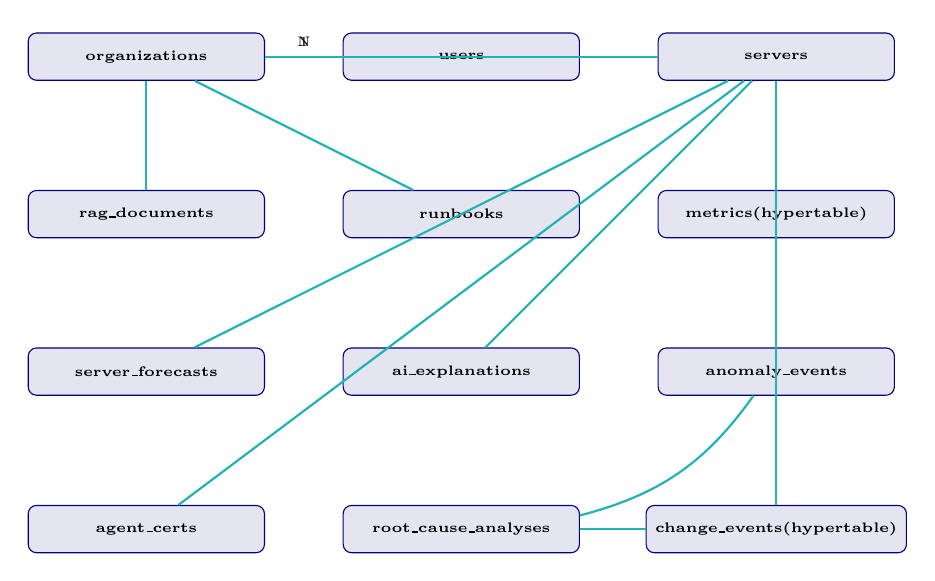
\begin{tikzpicture}[
  entity/.style={draw=NavyBlue, fill=NavyBlue!10, rounded corners=3pt,
    minimum width=3.0cm, minimum height=0.6cm, font=\tiny\bfseries},
  rel/.style={draw=TealBlue, thick},
  attr/.style={draw=DarkGray, fill=LightGray, minimum width=2.2cm,
    minimum height=0.4cm, font=\tiny}
]
% Entités
\node[entity] (org)   at (0, 6)    {organizations};
\node[entity] (usr)   at (4, 6)    {users};
\node[entity] (srv)   at (8, 6)    {servers};
\node[entity] (met)   at (8, 4)    {metrics\\(hypertable)};
\node[entity] (ano)   at (8, 2)    {anomaly\_events};
\node[entity] (aiexp) at (4, 2)    {ai\_explanations};
\node[entity] (fore)  at (0, 2)    {server\_forecasts};
\node[entity] (rag)   at (0, 4)    {rag\_documents};
\node[entity] (run)   at (4, 4)    {runbooks};
\node[entity] (chg)   at (8, 0)    {change\_events\\(hypertable)};
\node[entity] (rca)   at (4, 0)    {root\_cause\\\_analyses};
\node[entity] (cert)  at (0, 0)    {agent\_certs};

% Relations
\draw[rel] (org) -- node[above,font=\tiny]{1} (usr) -- node[above,font=\tiny]{N} (org);
\draw[rel] (org) -- (srv);
\draw[rel] (srv) -- (met);
\draw[rel] (srv) -- (ano);
\draw[rel] (srv) -- (aiexp);
\draw[rel] (srv) -- (fore);
\draw[rel] (srv) -- (chg);
\draw[rel] (srv) -- (cert);
\draw[rel] (ano) to[bend left=20] (rca);
\draw[rel] (rca) -- (chg);
\draw[rel] (org) -- (rag);
\draw[rel] (org) -- (run);
\end{tikzpicture}
\caption{Diagramme entité-association simplifié de \caimp{} (17 tables)}
\label{fig:erd}
\end{figure}

\section{Flux de traitement détaillés}

\subsection{Flux 1 : Ingestion de métriques}

L'agent collecte les métriques toutes les 15 secondes et les envoie au
Telemetry Writer via OTLP/HTTP. Le Telemetry Writer exécute les opérations
suivantes dans une goroutine Go :
\begin{enumerate}
  \item Décodage du batch OTLP et normalisation des noms de métriques
    (\texttt{system.cpu.utilization} → stocké tel quel) ;
  \item Insertion en bloc dans la table \texttt{metrics} via
    \texttt{COPY} PostgreSQL (batch de 2~000 lignes maximum) ;
  \item Passage des points au détecteur d'anomalies (trois algorithmes en
    parallèle) ;
  \item Publication de chaque anomalie détectée sur le sujet
    \texttt{anomaly.detected.\{org\_id\}.\{severity\}}.
\end{enumerate}

\subsection{Flux 2 : Corrélation de changements}

\begin{enumerate}
  \item Le Correlation Engine reçoit un message \texttt{anomaly.detected.*} ;
  \item Il exécute une requête SQL sur \texttt{change\_events} dans la fenêtre
    $[t - 30\text{min}, t]$ pour le même serveur ;
  \item Chaque changement est scoré :
    $s = e^{-0.1 \cdot \Delta t} \times w_{\text{type}}$,
    où $\Delta t$ est l'écart en minutes et $w_{\text{type}} \in [0.3, 1.0]$
    selon le type de changement ;
  \item Les trois changements de score le plus élevé sont envoyés à Ollama avec
    le contexte de l'anomalie ;
  \item Le résultat est persisté dans \texttt{root\_cause\_analyses} et publié
    sur \texttt{rootcause.ready.\{org\_id\}}.
\end{enumerate}

\section{Sécurité : modèle de menaces STRIDE}

L'analyse STRIDE (\textit{Spoofing, Tampering, Repudiation, Information Disclosure,
Denial of Service, Elevation of Privilege}) identifie les menaces suivantes et
les contre-mesures appliquées dans \caimp{} :

\begin{table}[H]
\centering
\caption{Analyse STRIDE et contre-mesures de \caimp{}}
\label{tab:stride}
\small
\begin{tabularx}{\textwidth}{lXX}
\toprule
\textbf{Menace} & \textbf{Exemple concret} & \textbf{Contre-mesure} \\
\midrule
Spoofing       & Agent malveillant envoyant des métriques falsifiées
               & Certificat mTLS ECDSA P-256 ; jeton JWT court \\
Tampering      & Modification des métriques en transit
               & TLS 1.3 ; intégrité AEAD \\
Repudiation    & Nier une action administrative
               & Journal d'audit immuable (\texttt{audit\_log}) \\
Info Disclosure& Accès aux données d'une autre organisation
               & RLS PostgreSQL ; isolation réseau Docker \\
DoS            & Flood de métriques depuis un agent compromis
               & Rate limiting Nginx (200~req/min/IP) \\
EoP            & Utilisateur \texttt{viewer} accédant aux routes admin
               & RBAC : vérification du rôle dans chaque endpoint \\
\bottomrule
\end{tabularx}
\end{table}

\section*{Conclusion}

Ce chapitre a présenté les fondations architecturales de \caimp{} : le choix
de l'architecture microservices, l'organisation des 19 services en quatre couches,
le bus d'événements NATS JetStream, le modèle de données relationnel et les
principaux flux de traitement. Cette architecture assure la séparation des
préoccupations nécessaire à l'évolutivité et à la maintenabilité de la plateforme.
Le chapitre suivant justifie les choix technologiques qui donnent corps à cette architecture.
